\section{The action of M�bius transformations}

So far we often talked about the action of M�bius transformations on $\EC$. However, up to now occasions have been quite rare where we literally could see them ``in action''. Maybe the most important exceptions to this are Figures~\ref{fig_StereoProjInversion} and \ref{fig_StereoProjModCayley}, showing continuous transitions between certain sets and their images under the two transformations $z \mapsto \reci{z}$ and  $z \mapsto \ModCayley(z)$ (the modified Cayley transform), both induced by rotations of the Riemann sphere. 

In this section we introduce a more direct method for visualization of such continuous transitions, a method working for arbitrary M�bius transformations and doing without stereographic projection and motion of Riemann spheres. For this purpose, we exploit the ``linear algebra nature'' (see Remark~\ref{rem_NatureMoebius}) of M�bius transformations. For easier notation we will not distinguish between a matrix $A \in \GL{\C}$ and the corresponding M�bius transformation ${}_\pm A \in \PGL{\C}$. In particular with $A$ we will denote both, a matrix and its associated transformation.

For $A \in \GL{\C}$ and $k \in \Z$, it follows from Theorem~\ref{thm_MoebiusGroup} that the matrix power $A^k$ corresponds to the M�bius transformation obtained by $k$ times composing the transformation $A$ with itself. The idea is now to generalize the concept of matrix powers from integral to real exponents. If we do so, then for any set $S \in \EC$ of interest, we can visualize the transition from $S$ to its image under $A$ simply by depicting a sequence of intermediate images $A^t S \subseteq \EC$, with a varying parameter $t \in [0,1]$.

\index{Generalized!matrix power}
In order to introduce such \emph{generalized matrix powers}, note that for integral exponents, powers of $A$ can be calculated by using its \index{Jordan normal form} \emph{Jordan normal form}.\footnote{Also called \emph{Jordan canonical form}. For more details on Jordan normal forms, eigenvalues and eigenvectors see for example \Hungerford{}, Chapter VII, Linear algebra.} If $J$ is a Jordan normal form of $A$, then for some $P \in \GL{\C}$ we have $A = \inv{P} J P$ and consequently
\begin{equation}
\label{eqn_MatrixIntPower}
A^k = \inv{P} J^k P, \quad\text{for all } k \in \Z.
\end{equation}
The matrix $J$ has one of the two possible forms
\begin{equation*}
(i)\ J = \mat{\lambda_1}{0}{0}{\lambda_2} \quad\text{or}\quad 
(ii)\ J = \mat{\lambda}{1}{0}{\lambda}
\end{equation*}
and their respective matrix powers are given by
\begin{equation}
\label{eqn_JordanPower}
(i)\ J^k = \mat{\lambda_1^k}{0}{0}{\lambda_2^k} \quad\text{or}\quad
(ii)\ J^k = \mat{\lambda^k}{k \lambda^{k-1}}{0}{\lambda^k}.
\end{equation}
From here it is just a small step to the generalization of matrix powers to real exponents: We choose a fixed branch of the natural (complex) logarithm, for example such that the imaginary part of the logarithm ranges in the interval $(-\pi,\pi]$, \ie $\Im{\ln z} = \arg z \in (-\pi,\pi]$ for all $z \in \C$. Now, for $\lambda \in \C$ and $k \in \R$, we can evaluate $\lambda^k$ as $\lambda^k := \exp(k \ln \lambda)$.

\begin{definition}[Generalized matrix power]
\label{dfn_GenMatPower}
Let $A \in \GL{\C}$ be a matrix. For $k \in \R$ we say $B$ is an $k$-th power of $A$, in symbols $B = A^k$, if there is a $P \in \GL{\C}$ such that
\begin{equation*}
A = \inv{P} J P \quad \text{and} \quad B = \inv{P} J^k P,
\end{equation*}
where $J$ is in Jordan normal form and $J^k$ is determined by (\ref{eqn_JordanPower}), where a fixed branch of the natural logarithm is chosen and the expressions $\lambda^k$ are evaluated as $\lambda^k := \exp(k \ln \lambda)$.
\end{definition}

\begin{remark}[Eigenvectors and fixed points]
Writing the matrix $P$ in the form $P = (v_1 \mid v_2)$ with $v_1, v_2 \in \C^2$, in case $(i)$, $v_1$ and $v_2$ are the \index{Eigenvector} \emph{eigenvectors} of the matrix $A$ corresponding to the \index{Eigenvalue} \emph{eigenvalues} $\lambda_1$ and $\lambda_2$ respectively. In case $(ii)$, only $v_1$ is an eigenvector ($v_2$ is a so-called \index{Generalized!eigenvector} \emph{generalized eigenvector}). It is worth noting that a vector $({}^u_v) \in \C^2$ is an eigenvector of $A \in \GL{\C}$, if and only if $u/v \in \EC$ is a fixed point for the M�bius transformation $A$:
\begin{equation*}
A \cdot \cvec{u}{v} = \lambda \cvec{u}{v} \quad\Leftrightarrow\quad
A \left(\frac{u}{v}\right) = \frac{\lambda u}{\lambda v} = \frac{u}{v}.
\end{equation*}
Therefore, in case $(i)$, $A$ is either the identity transformation or has exactly two distinct fixed points in $\EC$. In case $(ii)$, $A$ has exactly one fixed point in $\EC$.
\end{remark}

As Definition~\ref{dfn_GenMatPower} already suggests, generalized matrix powers are not unique but depend on the chosen branch of the natural logarithm. The following example will illustrate this:
\begin{example}
\label{ex_InversionSqrt}
Let $A = \smallmat{0}{1}{1}{0} \in \GL{\C}$ be the matrix corresponding to the M�bius map $z \mapsto \reci{z}$. We wish to calculate the ``square root'' $A^{\reci{2}}$ of this transformation. The eigenvalues of $A$ are $\lambda_1 = -1$ and $\lambda_2 = 1$; the corresponding eigenvectors are $v_1 = ({}^{-1}_{\phantom{+}1})$ and $v_2 = ({}^1_1)$. We can therefore write $A$ as
$A = \inv{P} J P$ with $P = \smallmat{-1}{1}{\phantom{+}1}{1}$ and $J = \smallmat{-1}{0}{\phantom{+}0}{1}$.
Next we calculate $J^{\reci{2}}$ by evaluating $\exp(\reci{2} \ln \lambda_1)$ and $\exp(\reci{2} \ln \lambda_2)$. Choosing a logarithm branch such that $\Im{\ln z} \in (-\pi,\pi]$ for all $z \in \C$, and denoting equivalence of matrices in $\PGL{\C}$ again by $\sim$, this yields $J^{\reci{2}} = \smallmat{\ii}{0}{0}{1}$ and
\begin{equation*}
A^{\reci{2}} = \inv{P}J^{\reci{2}}P = \reci{2} \mat{1+\ii}{1-\ii}{1-\ii}{1+\ii} \sim \mat{\ii}{1}{1}{\ii}.
\end{equation*}
We therefore see that $A^\reci{2} = \ModCayley$ and the modified Cayley transform is in this sense a ``square root'' of the transformation $A : z \mapsto \reci{z}$ -- compare also Example~{\ref{ex_ModCayleyTransform}}.

In contrast to that, choosing a slightly different logarithm branch, such that $\Im{\ln z} \in [-\pi,\pi)$ for all $z \in \C$, we get $J^{\reci{2}} = \smallmat{-\ii}{0}{\phantom{+}0}{1}$ and therefore obtain a matrix conjugate to the above one:
\begin{equation*}
A^{\reci{2}} = \reci{2} \mat{1-\ii}{1+\ii}{1+\ii}{1-\ii} \sim \mat{-\ii}{1}{1}{-\ii}.
\end{equation*}
Note that this second transformation, just like the modified Cayley transformation, can also be considered as a quarter-turn of the Riemann sphere around the $x_1$ axis, but it rotates in the opposite direction and maps the \emph{lower} half-plane to the unit disk.
\end{example}

\begin{example}
As an application of generalized matrix powers, we can visualize the action of the modular transformations $U : z \mapsto z+1$, $T: z \mapsto -\reci{z}$ and $R: z \mapsto -\reci{z+1}$ on the modular tessellation. For the parameter $t \in [0,1]$ ``intermediate actions'' of these maps are given through the M�bius maps corresponding to the matrices
\begin{eqnarray*}
U^t &\sim& \mat{1}{t}{0}{1},\\
T^t &\sim& \mat{\cos \left(\frac{\pi t}{2}\right)}{-\sin \left(\frac{\pi t}{2}\right)}{\sin \left(\frac{\pi t}{2}\right)}{\cos \left(\frac{\pi  t}{2}\right)},\\
R^t &\sim& \mat{\sqrt{3} \cos \left(\frac{\pi t}{3}\right)-\sin \left(\frac{\pi t}{3}\right)}{-2 \sin \left(\frac{\pi t}{3}\right)}{2 \sin \left(\frac{\pi t}{3}\right)}{\sqrt{3} \cos \left(\frac{\pi t}{3}\right)+\sin \left(\frac{\pi t}{3}\right)}.
\end{eqnarray*}

In Figures~\ref{fig_UAction}, \ref{fig_TAction} and \ref{fig_RAction} we can see the modular tessellation and its ``intermediate images'' under the transformations $T$, $U$ and $R$ for the parameter values $t \in \{0, \reci{5}, \frac{2}{5}, \frac{3}{5}, \frac{4}{5}, 1\}$. Again we use the modified Cayley transform to map the tessellation of the upper half-plane to the unit disk. Looking at Figure~\ref{fig_TAction}, another advantage of seeing the upper half-plane from this different angle gets apparent: Under $\ModCayley$, the action of $T$ corresponds to a simple rotation by $180^\circ$ around the fixed point $\ii$. This is in close connection to Remark~\ref{rem_TRotation}, where we noted that $T$ corresponds to a half-turn of the Riemann sphere around the $x_2$ axis. Finally we can see in Figure~\ref{fig_RAction} that -- with a slight distortion -- $R$ corresponds to a rotation by $120^\circ$ around the fixed point $\rho = \exp(2 \pi \ii / 3)$.

Note that the individual frames in Figures~\ref{fig_UAction}, \ref{fig_TAction} and \ref{fig_RAction} have been arranged such that the first column has to be read first in top-down direction and then the second column has to be read in bottom-up direction, allowing in the first row a direct comparison of the original tessellation and its image under the respective transformations.
\begin{figure}
\centering
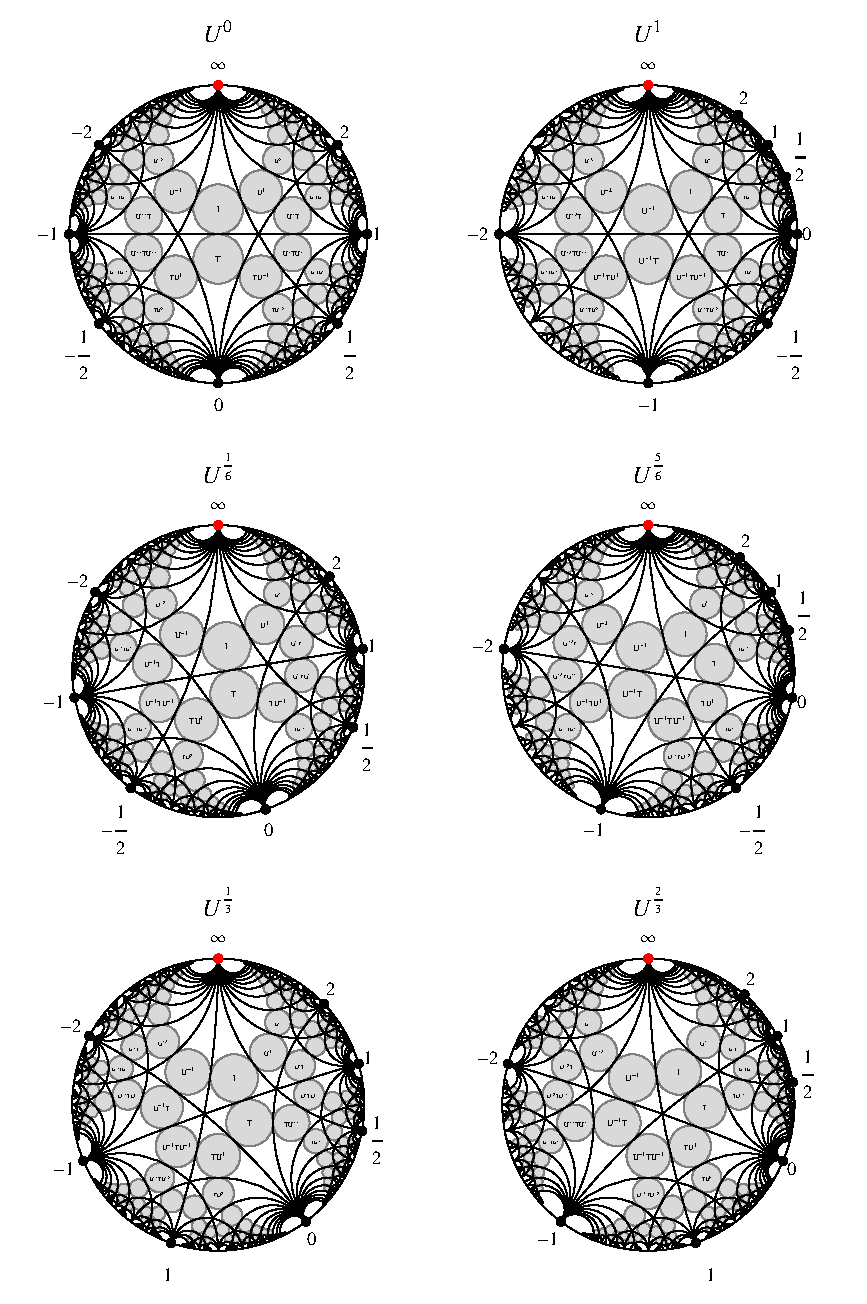
\includegraphics[width=0.98\textwidth]{figures/u-action}
\caption{The action of $U : z \mapsto z+1$.}
\label{fig_UAction}
\end{figure}

\begin{figure}
\centering
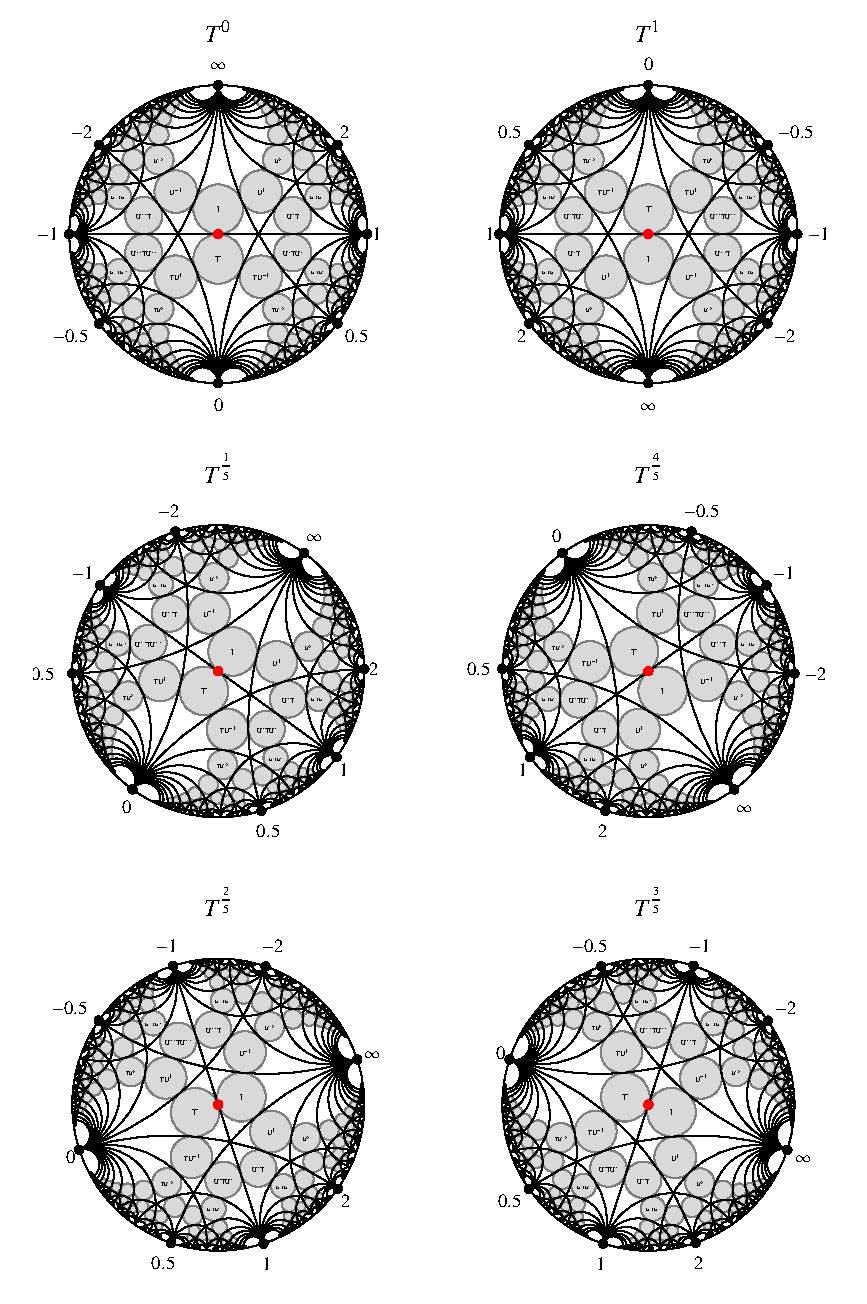
\includegraphics[width=0.98\textwidth]{figures/t-action}
\caption{The action of $T : z \mapsto -\reci{z}$.}
\label{fig_TAction}
\end{figure}

\begin{figure}
\centering
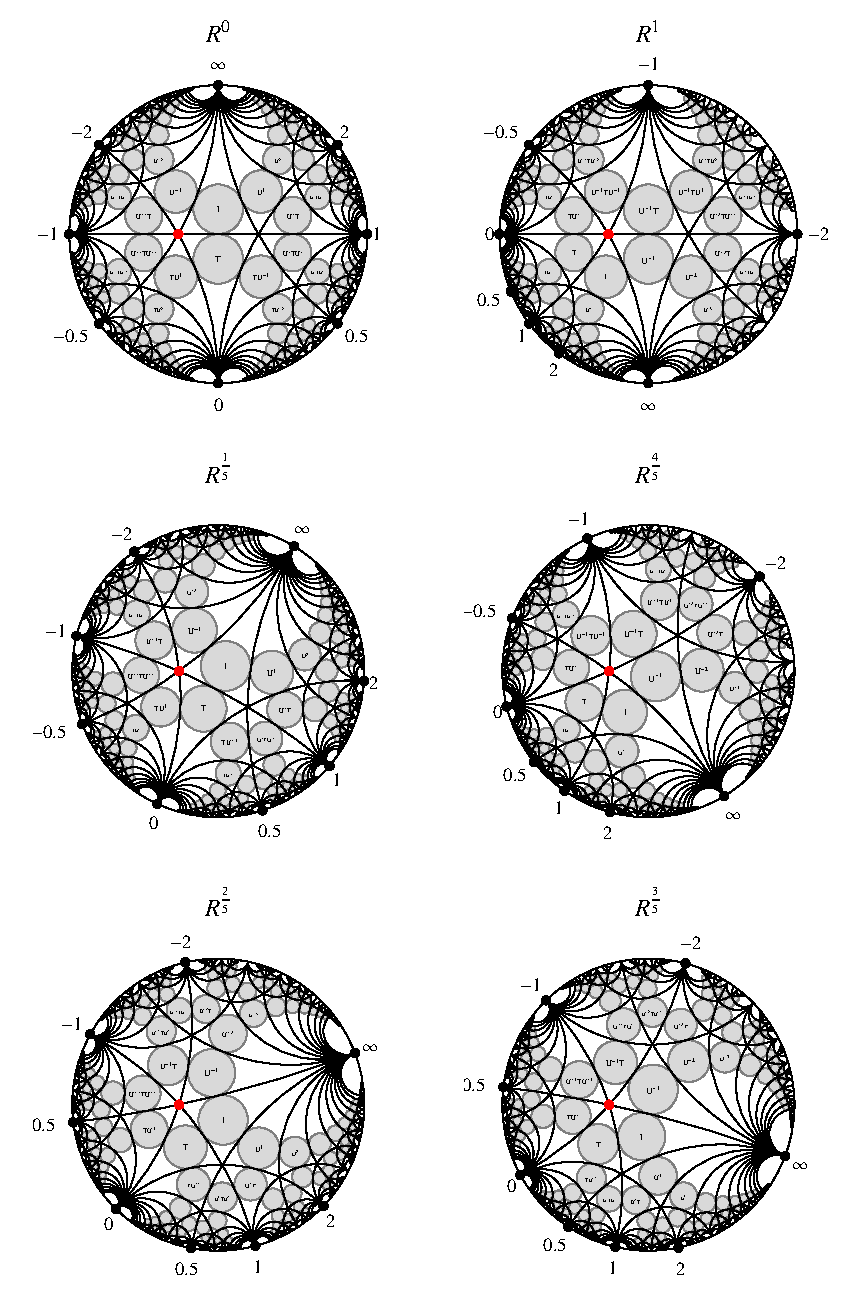
\includegraphics[width=0.98\textwidth]{figures/r-action}
\caption{The action of $R : z \mapsto -\reci{z+1}$.}
\label{fig_RAction}
\end{figure}
\end{example}
\clearpage
